\documentclass[11pt,a4paper,slovene]{myarticle}

%Uporabljeni paketi
\usepackage[slovene]{babel}
\usepackage[utf8]{inputenc}
\usepackage{lmodern}
\usepackage[T1]{fontenc}
\usepackage{fancyhdr}
\usepackage{caption}
\captionsetup{font={default,footnotesize}, labelfont=bf, format=hang,indention=.0cm}
\usepackage{graphicx,epsfig}
\usepackage{amsmath}
\usepackage{multirow}
\usepackage{color}
\usepackage{url}
\usepackage{makeidx}
\usepackage[official]{eurosym}
\usepackage{float}
\usepackage{hyperref}
\hypersetup{
   bookmarksnumbered=true,
   urlbordercolor={0 1 0},
   linkbordercolor={1 1 1},
   unicode=true,
   pdftitle={ Modeliranje Računalniških Omrežij },
   pdfauthor={Asistent},
   pdfdisplaydoctitle=true,
   pdftoolbar=true,
   pdfmenubar=true,
   pdfstartview=X Y Z
}

\urlstyle{same}

\setlength{\parskip}{12pt}
\setlength\parindent{0pt}
\setlength\unitlength{1mm}

\begin{document}
\label{naslov}
\pdfbookmark[1]{Naslov}{naslov}
\thispagestyle{empty}

\begin{center}
\begin{Large}
Modeliranje računalniških omrežij\\
Študijsko leto 2013/2014\\
\end{Large}

\vspace*{4cm}
\begin{LARGE}
\textbf{Modeliranje IPv6 omrežij\\}
\end{LARGE}
\vspace*{0.5cm}

\begin{Large}
1. delno poročilo velike seminarske naloge\\

\vspace*{4cm}

Nihad Kerić, 63099999\\
Miha Novak, 63100268\\
Gregor Bahor, 63090049\\
Darko Janković, 63100176\\

\vspace*{5cm}
Ljubljana, \today
\end{Large}
\end{center}

\pagebreak
\setcounter{page}{1}
\pagenumbering{arabic}


\label{Kazalo}
\pdfbookmark[1]{Kazalo}{Kazalo}
\tableofcontents
\thispagestyle{empty}
\pagebreak

\section{Naloga}
Modelirajte bolj kompleksne primere IPv6 omrežja s pomočjo INET ogrodja v orodju OMNeT++. 

\section{Opis 3 zgledov za modeliranje IPv6 omrežij v INET ogrodju.}
\subsection{Pv6NClients}
V datoteki NclientsEth.ned oz. NclientsPPP.ned imamo skonfigurirano omrežje s tremi IPv6 usmerjevalniki ter n IPv6 odjemalcev(komuniciranje preko aplikacije TelnetApp). Ipv6 odjemalci so strežnik in n klienti, kar je prikazano na sliki spodaj. Stevilo n-klientov v našem testnem primeru se doloci v konfiguraciji :[General]*.n=10, lahko tudi spremenimo čas izvajanja simulacije v nasem primeru 'sim-time-limit=168h' v datoteki omnetpp.ini. Vsi klienti so vezani na en usmerjevalnik r1. Med klienti in strežnikom so med seboj zaporedno vezani trije usmerjevalniki, strežnik je vezan na usmerjevalnik r3. Ob zagonu simulacije se vzpostavi stanje omrežja, nato pa se prične seja med strežnikom in klienti. Seje se izmenjujemo med razlicnimi klienti. Pri testiranju različno velikem številu klientov n=2,10,100,200 in pri simulacijskem času 168h ni prišlo do napak.Simulacija NClientsPPP je identična po zgradbi omrežja NclientsEth.
Razlika med omrežjema se pojavi v načinu povezave fiberline ali ethernetline in stem se spremeni cas potovanja paketov in propustnost kanalov.
Simulacija NclientsEth ima definirano hitrost prenosa podatkov datarate=100Mbps in je počasnejša od NClientsPPP, katera ima hitrost prenosa podatkov datarate=1Gbps.

\subsection{IPv6Bulk}
Omrežje sestavljajo strežnik, usmerjevalnik in trije odjemalci. Strežnik in vsi trije odjemalci so povezani z usmerjevalnikom, obstaja pa tudi direktna povezava med strežnikom in enimi izmed odjemalcem. Vse povezave so tipa in/out, hitrost prenosa podatkov po kanalu pa je 10Mbps z zakasnitvijo 0.1us. Ves promet v omrežju usmerja usmerjevalnik, ki usmerja tudi promet med strežnikom in odjemalcem. 
\\
Pred zagonom simulacije lahko izbiramo med različnimi implementacijami TCP
(Transmission Control Protocol):
\begin{itemize}
\item TCP, je protokol za nadzor prenosa podatkov, ki zagotavlja, da se informacije med prenosom ne izgubijo, ne spremenijo in da se informacije vnovič dostavijo, če je prišlo med prenosom do napake.
\item TCP\_lwIP, TCP lightweight IP, je široko uporabljen odprtokodni TCP/IP protokolni sklad oblikovan za uporabo v vgrajenih sistemih.
\item TCP\_NSC, implementacija TCP, ki je bila razvita v okviru NSC projekta (Network Simulation Cradle project)
\end{itemize} 
Opazujemo lahko izvajanje NDP (Neighbor Discovery Protocol) in TCP seje (trosmerno rokovanje, prenos podatkov).
\\
Paketi, ki se prenašajo pri NDP (Neighbor Discovery Protocol):
\begin{itemize}
\item RSpacket (Router Solicitation)
\item RApacket (Router Advertisement)
\item NSpacket (Neighbour Solicitation)
\item NApacket (Neighbour Advertisement)
\end{itemize}
Paketi, ki se prenašajo pri TCP seji
\begin{itemize}
\item SYN
\item SYN + ACK
\end{itemize}

\subsection{Nclients}
Nclient ima dve mreži :
1) NClientsEth.ned
2) NClientsPPP.ned

\subsubsection{NClientsEth}
Pri tistem omrežiju imamo komunikaciju med odjemalcem in strežnikom,ali pač z n odjemalcov pa enim strežnikom preko 3 usmerjevalnika. Kateri so povezani preko  ipv6 protokola, naslovi so razdelni na 8 naslovo.
V NClientsEth.ned fielu imam dve vrsti kanalov (channel):
- fiberline
-ethernetline
Kanali imata iste antribute z različnimi nastavitvi.
            fiberline (delay= 1us in datarate= 512 Mbps)
ethernetline (delay= 0.1us in datarate= 10 Mbps)
Usmerjevalniki komunicirajo preko tistih kanalov ,prvo uspostave povezavo pošiljanjem različnih paketov kot so: NSpacket  , RApacket, RSpacket  , SYN, SYN+ACK. Po vzpostavljenoj povezavi se začneju pošiljati paketov. Strežnik pošlje paket proti odjemalcu kateri pol odgovori z pošiljanjem paketa ACK.  Isto se zgodi pri pošiljanu paketov z strani odjemalca.

\subsubsection{NClientPPP}
Tudi v tem omrežiju imamo komunikaciju med n odjemalcev in strežnikom preko tri usmerjevalnika, ipv6 naslov je razdelen na 8 naslovo kateri so krajši od naslovo prve konfiguracije v temu se razlikujeta.
 V NClientsEth.ned fielu imam  kanal (channel):
            -fiberline z nastavitvemi: (delay= 1us in datarate= 512 Mbps)
 

\section{Podrobna analiza enega od zgledov}
Za analizo smo izbrali zgled \textit{demonetworketh}.
\begin{figure}[H]
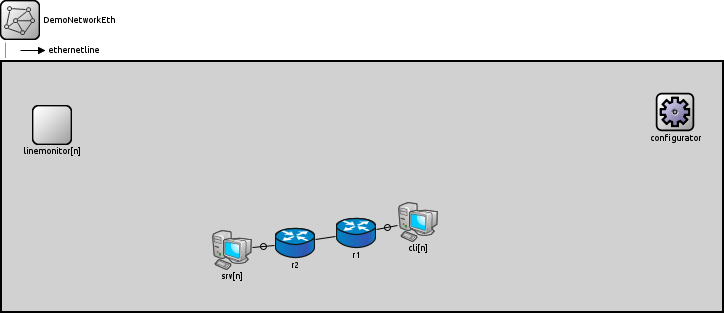
\includegraphics[scale=0.5]{slike/demoNetworkEth.png}
\end{figure}
Omrežje je sestavljeno iz naslednjih gradnikov:
\begin{itemize}
\item configurator tipa FlatNetworkConfigurator6
\item r1 tipa Router6
\item r2 tipa Router6
\item cli[n] tipa StandardHost6
\item srv[n] tipa StandardHost6
\item linemonitor[n] tipa TCPDump
\end{itemize}

\textbf{FlatNetworkConfigurator6}\\
Konfigurira Ipv6 naslove in posredovalne tabele.

\textbf{Router6}\\
Predstavlja Ipv6 usmerjevalnik.

\textbf{StandardHost6}\\
Ipv6 gostitelj s TCP, SCTP in UDP plastmi in aplikacijami.

\textbf{TCPDump}\\
Pregledovanje vsebine paketov.

\section{Podroben opis razpoložljivih gradnikov INET ogrodja}
Opisali smo gradnike iz primera \textit{demonetworketh}.

\subsection{NetworkLayer6}
Omrežje vsebuje elemente, ki so ključnega pomena pri klientih, usmerjevalnikih in strežnikih.
Modul NetworkLayer6.ned predstavlja Ipv6 omrežno plast in  je sestavljen iz elementov:
-import inet.networklayer.ipv6.IPv6ErrorHandling;
-import inet.networklayer.ipv6.IPv6;
-import inet.networklayer.icmpv6.IPv6NeighbourDiscovery;
-import inet.networklayer.icmpv6.ICMPv6;
\\
SLIKA
\\

-Ipv6: modul setavlja klasifikacijski obrejkt (modul) IPv6Datagram, ki predstavlja glavo
paketa IPv6 protokola. Ko modul ipv6 pošlje paket višjemu nivoju (TCP ali UDP
protokol) po ISO/OSI omrežnem modelu ga opremi z izvornim in ponornim naslovom.
Opisani elementi povezujejo 3. omrežni (IPv6) in 4. transportni (TCP/UDP) nivo po
OSI/ISO omrežnem modelu.
\\
-IPv6ErrorHandling:Napake pridejo v obliki sporočila, modul se uporablja za beleženje napak na omrežnem nivoju.
\\
-NeighburDiscovery: modul se uporablja za izvajanje vseh naloge, povezanih z odkritje
sosedov in brez naslovno auto konfiguracijo. Neighbour discovery paketi so sami poslani in obdelani stem modulom. Ko Ipv6 prejme enega, posreduje paket naprej k IPv6 Neighbor Discovery.
\\
-Icmpv6: modul, ki služi za pošiljanje zahtev »echo request« na omrežnem
nivoju. Zahteva bo poslana na vrat pingIn z proloženo IPv6ControlInfo. Odgovor »echo reply« bo sprejet, ko sporočilo bo poslano skozi vrata pingOut.

%\section{Zaključek}
%Ali ste izpolnili cilje in možne nadaljne nadgradnje. Pri %samem opisu rešitve se običajno sklicujemo na reference, npr. %\cite{omnetpp} in \cite{cisco}. 

\pagebreak
\bibliographystyle{plain}
\bibliography{references}

\end{document}











